\documentclass[10pt]{exam}
\usepackage[utf8]{inputenc}		% Caracteres latinos
\usepackage[spanish]{babel}		% Idioma español
\usepackage{geometry}			% Organizar el documento
\usepackage{graphicx}			% Incluir gráficos
\usepackage{makecell}			% Para personalizar las celdas de una tabla
\usepackage[nohdr]{mathexam}	% Añadimos el paquete mathexam (sin header)
\usepackage{amsmath}
\usepackage{amsfonts}
\usepackage{amssymb}
\usepackage{mathtools}
\usepackage{tikz,pgfplots}
\usepgfplotslibrary{polar}
\usepackage[shortlabels]{enumitem}
\usepackage{textpos}
\usepackage{caption}
\usepackage{mwe}

 \renewcommand{\baselinestretch}{1.5}

%\usepackage[]{mathptmx}        % A free version o Times Roman with mathematical symbols
%\usepackage{pzc}               % fuente cursiva (conjuntos) Zapf Chancery
%\usepackage{showframe}
%\usepackage{lipsum}

% DOCUMENTACIÓN DE LA CLASE EXAM
% http://ftp.inf.utfsm.cl/pub/tex-archive/macros/latex/contrib/exam/examdoc.pdf
% DOCUMENTACIÓN DE LA CLASE MATHEXAM
% http://ctan.dcc.uchile.cl/macros/latex/contrib/mathexam/doc/mathexam.pdf

% Definimos la geometría de la primera página
\geometry{
	a4paper,                    % Tamaño del documento
	hmargin = {1.5cm, 1.5cm}, 	% Margen horizontal izquierdo, derecho
	vmargin = {1.5cm, 1cm},	    % Margen vertical superior, inferior
	headsep = 4mm,				% Separación entre el encabezado y el texto
	head = .2cm,				% Tamaño del encabezado
	% marginparsep = 5mm, 		% Seperación entre las notas y el texto
	% marginpar = 1.5cm,		% Tamaño de las notas
	includeall,                 % incluye el encabezado, footer y notas dentro del tamaño del documento
	nomarginpar,	            % Elimina las notas
	foot = 1cm,                 % Tamaño del footer
	twoside,                	% Habilita el modo de impresión a doble cara
}

\selectlanguage{spanish}        % Selecciona el idioma
\spanishdecimal{.}

%\pagestyle{headandfoot}         % Nuestro examen tendrá encabezado y pié

% DEFINIMOS EL ENCABEZADO
%\header{
%\begin{tabular}{l c c c l}
%            \makecell{\includegraphics[height=2.5cm]{logo.png}} &
%            \makecell{\textbf{IPEA 215} \\Raúl Scalabrini Ortiz} &
%            \makecell{Examen} &
%            \makecell{Curso\\1er Año} &
%             \makecell[l]{Apellido y %Nombre:\enspace\makebox[2in]{\hrulefill}\\Fecha: \today}
%        \end{tabular}}{}{}

% DEFINIMOS EL PIE
%\rfoot{Página \thepage\ de \numpages}

% DOCUMENTO
\begin{document}

\centering


\Large 
\textbf{Tarea 3}

\normalsize
Fecha de entrega: 

Miércoles 16/10/2024 durante la clase




\pointpoints{punto}{puntos}
\pointformat{\bfseries\boldmath(\thepoints)}
\vskip10pt

\begin{questions}
%    \question Correlaciona la gráfica de cada función dada en las figuras \textbf{(a)}-\textbf{(d)} con las gráficas de sus derivadas en las figuras \textbf{I} a \textbf{IV}. Explica las razones de cada selección.
%    \begin{center}
%    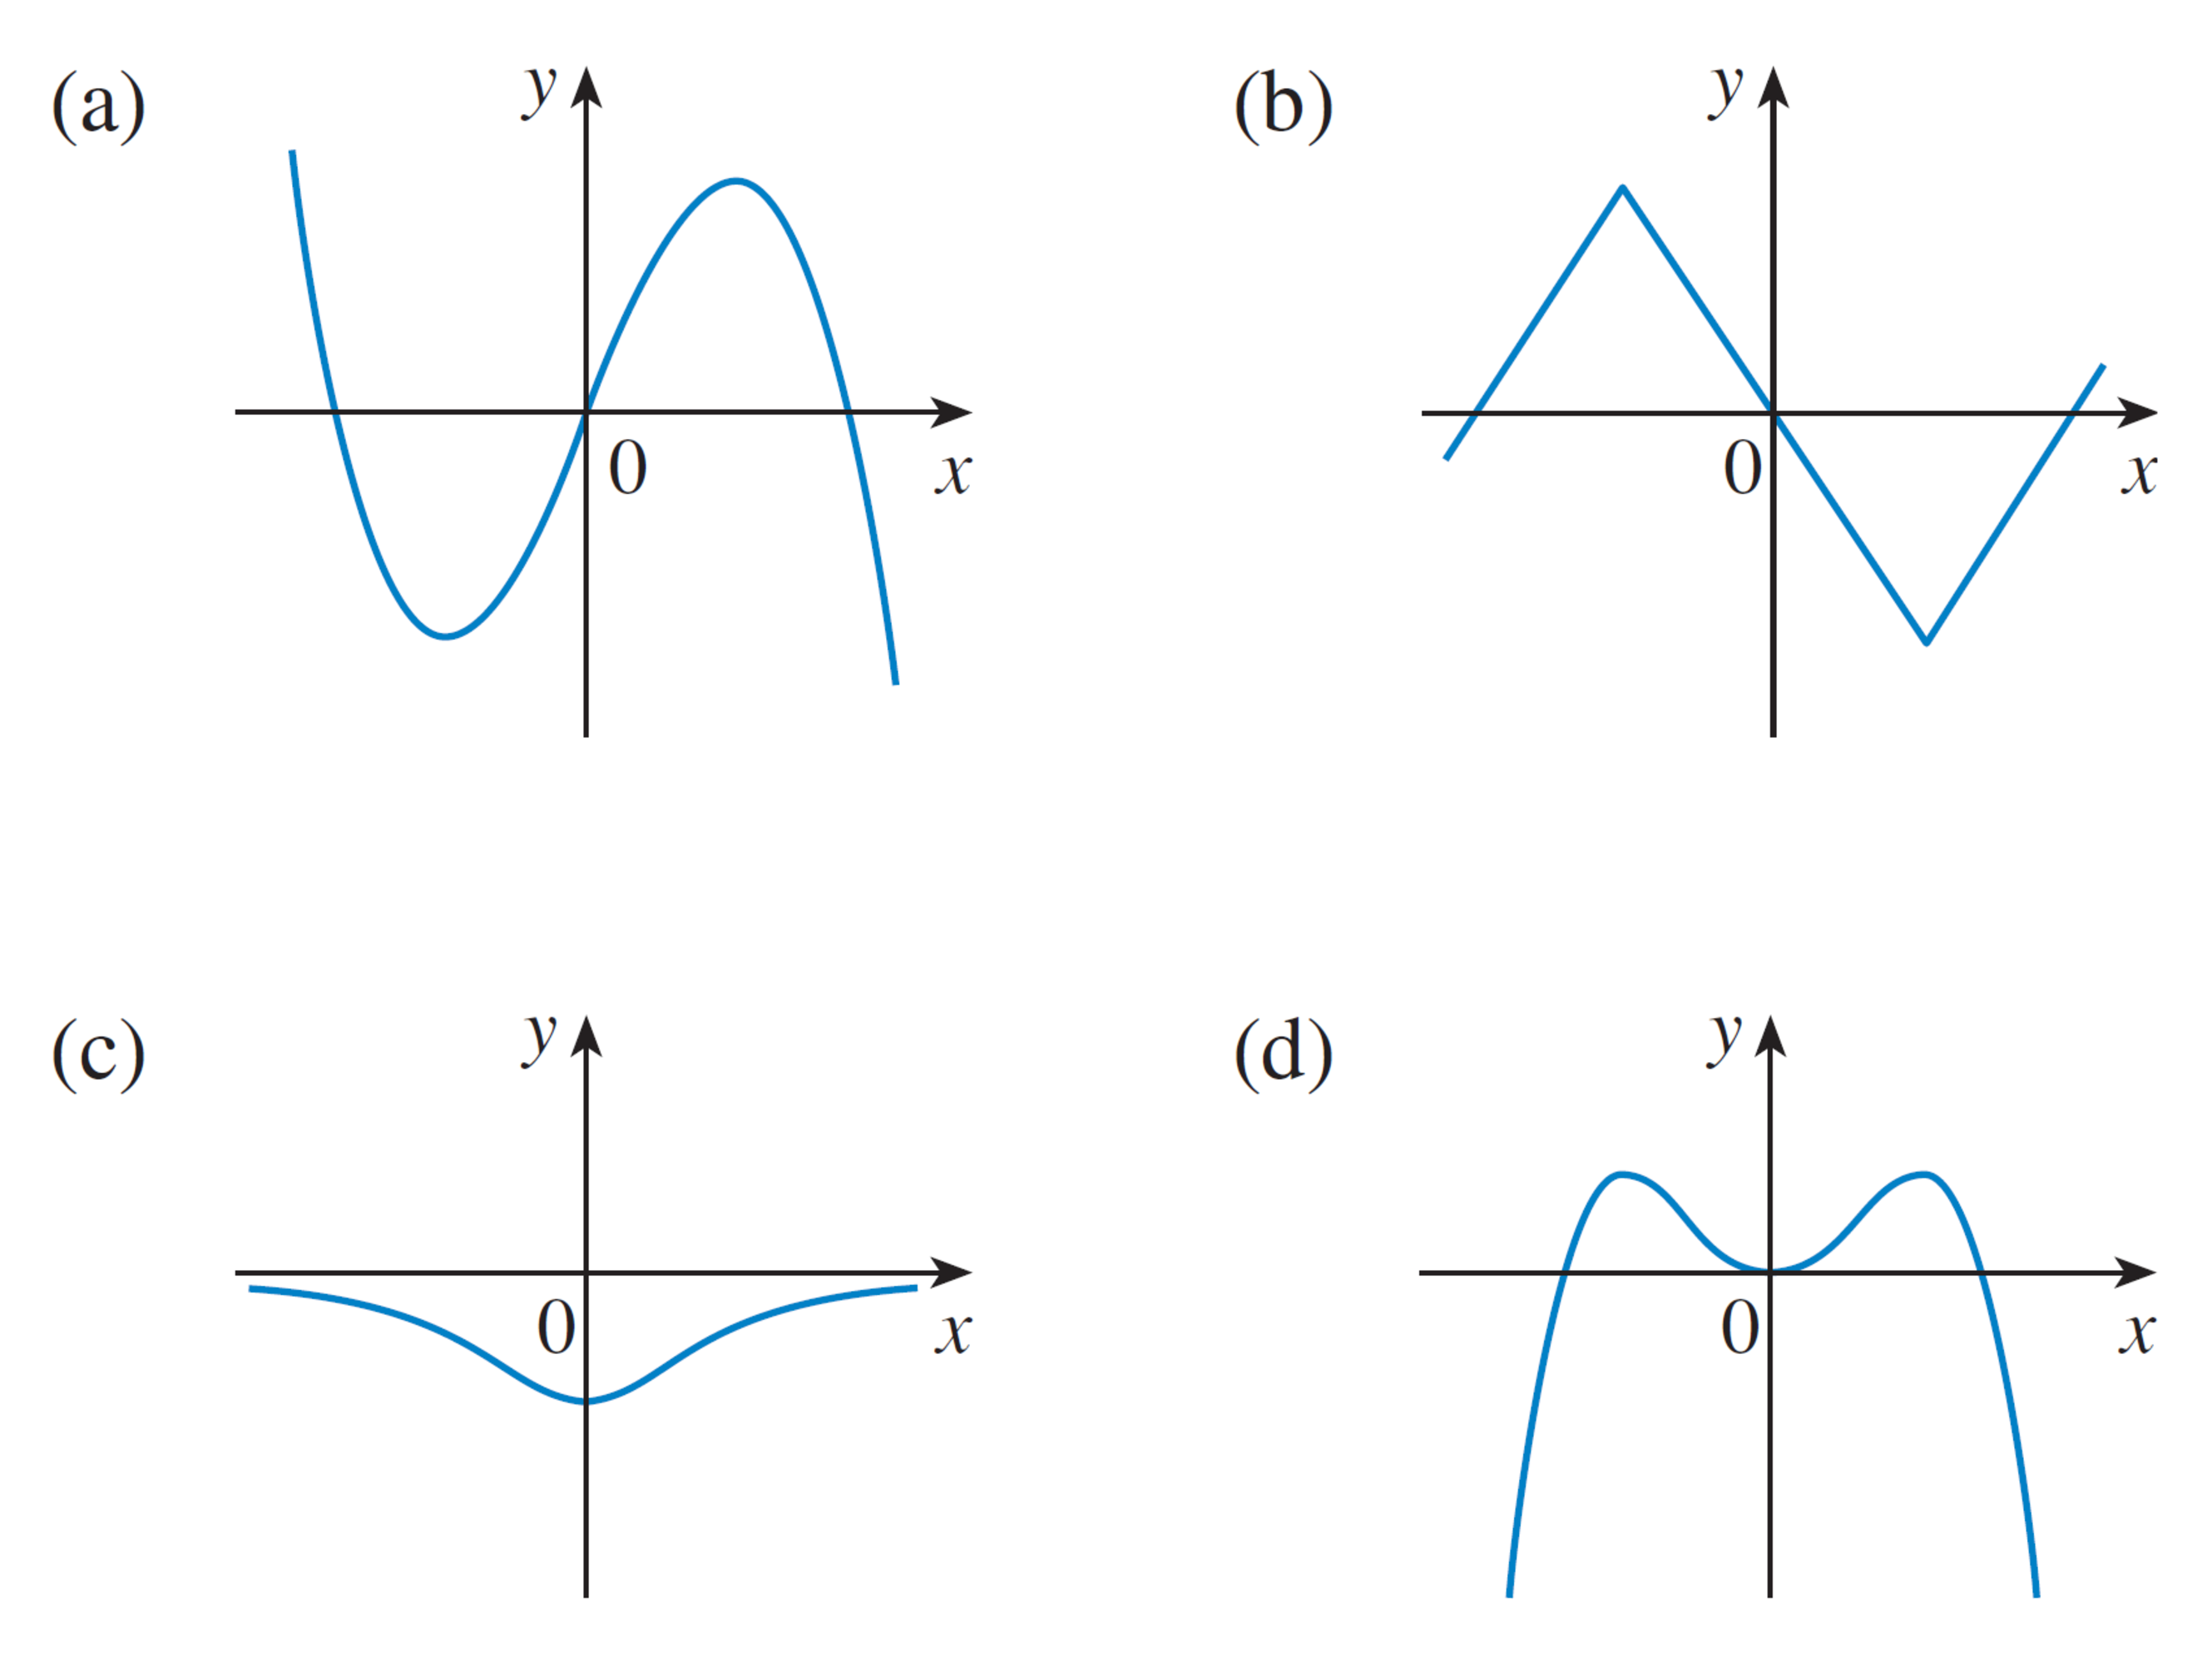
\includegraphics[width=6cm,height=4.5cm]{Graf1T-E.pdf}
%    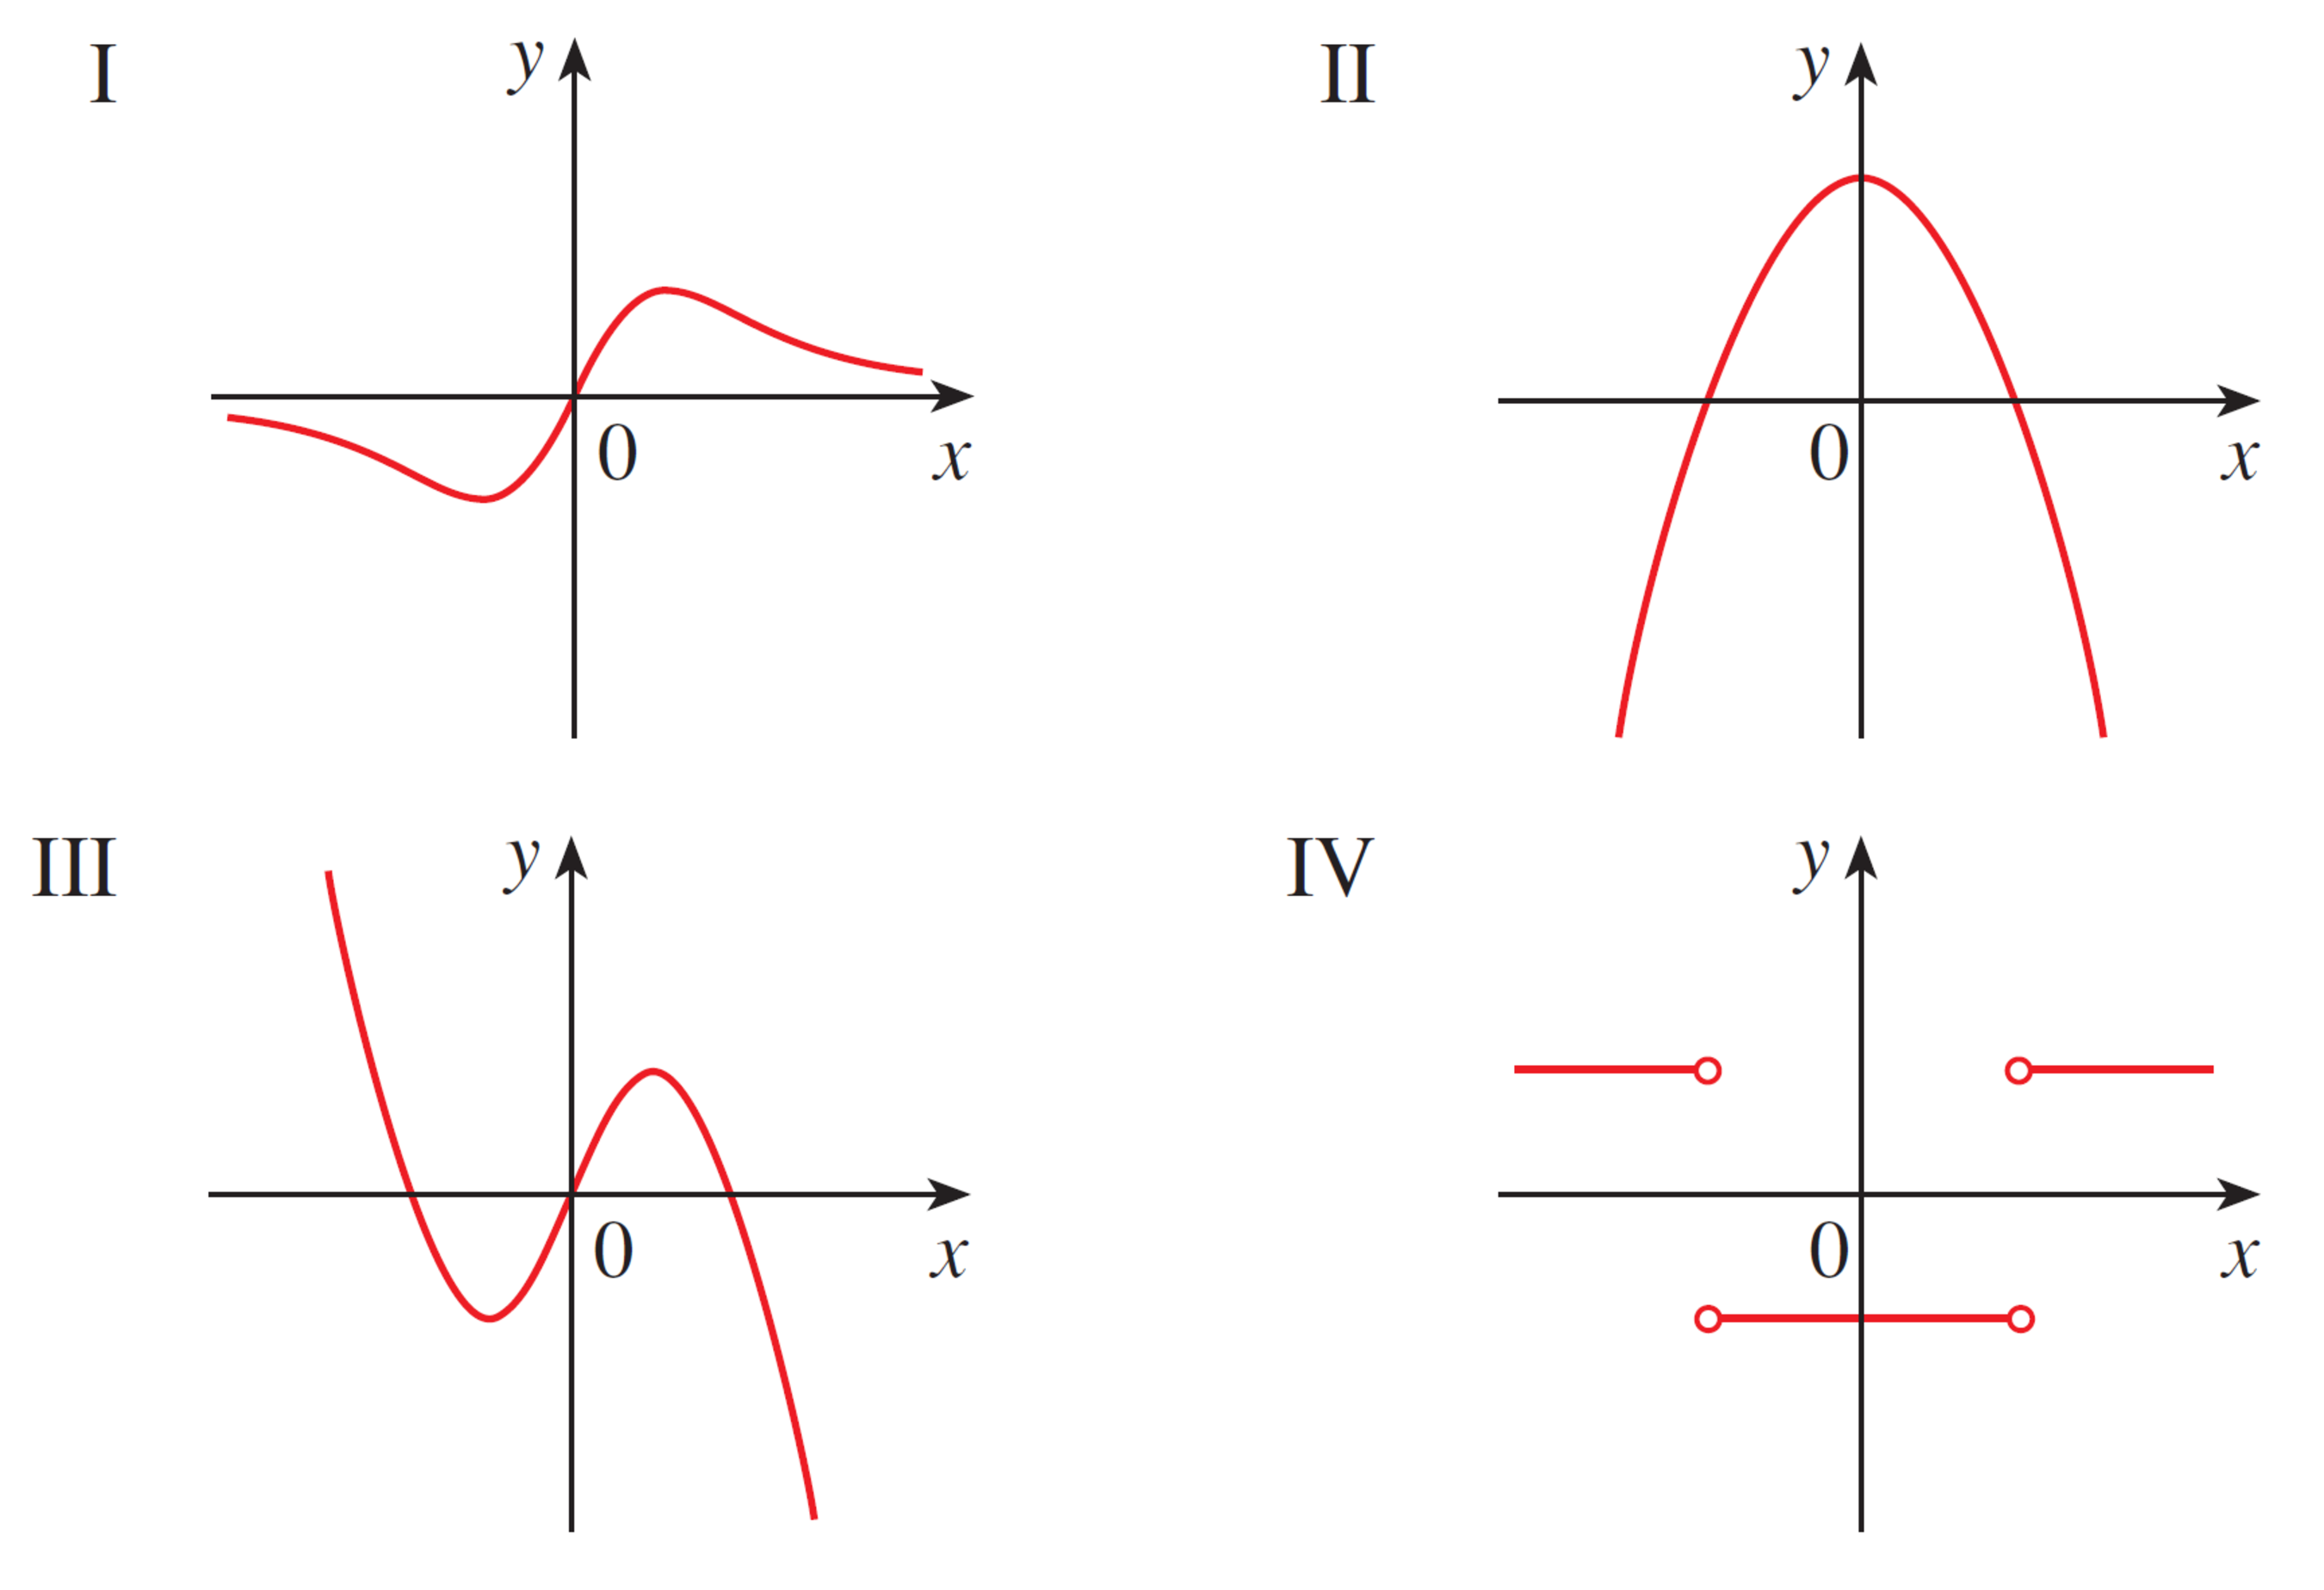
\includegraphics[width=6cm,height=4.5cm]{Graf2T-E.pdf}
%    \end{center}{}
    
%    \vskip15pt
%    \begin{textblock}{10}(8.4,.1)
%    \includegraphics[width=4.5cm,height=3cm]{Graf3T-E.pdf}
%    \end{textblock}  
%    \question De la gráfica $g(x)$ en la figura de la derecha:
%    \begin{enumerate}[a)]
%        \item ¿En cuáles números $g$ es discontinua? ¿Por qué?
%        \item ¿En cuáles números $g$ no es diferenciable? ¿Por que?
%    \end{enumerate}{}
%\vskip15pt

    \question La frecuencia de las vibraciones de una cuerda de un violín se expresa por medio de
$$f=\frac{1}{2L}\sqrt{\frac{T}{\rho}}$$
donde $L$ es la longitud de la cuerda, $T$ es su tensión y $\rho$ es su densidad lineal. Encuentra la rapidez de cambio de la frecuencia con respecto a:
\begin{itemize}
    \item La longitud (cuando $T$ y $\rho$ son constantes)
    \item La tensión (cuando $L$ y $\rho$ son constantes)
    \item La densidad lineal (cuando $L$ y $T$ son constantes)
\end{itemize}{}

El tono de una nota (qué tan alto o bajo suena) está determinado por la frecuencia $f$ (entre más alta la frecuencia más alto es el tono). Usa los signos de las derivadas obtenidas anteriormente para hallar qué sucede en el tono de una nota:
\begin{itemize}
    \item Cuando se disminuye la longitud efectiva de una cuerda colocando un dedo sobre la una cuerda de modo
que vibre una parte más corta de la misma.
    \item Cuando se aumenta la tensión haciendo girar una de las clavijas.
    \item Cuando se incrementa la densidad lineal al hacer sonar otra cuerda.
\end{itemize}{}

%\newpage
\vskip15pt

    \question Usando la definición formal de derivada $\left(f'=\lim\limits_{h \to 0}\frac{f(x+h)-f(x)}{h}\right)$ demuestra que:
    $$\frac{d}{dx}(e^x)=e^x \quad \text{usando y demostrando que} \quad 
       \lim\limits_{h\to0}\frac{e^h-1}{h}=1$$
    
%       \begin{enumerate}[i)]
%       \item $\frac{d}{dx}(\text{sen}\, x)=\text{cos}\,x$
%       \item $\frac{d}{dx}(\text{cos}\, x)=-\text{sen}\,x$
%       \item $\frac{d}{dx}(e^x)=e^x$ usando que
%       $\lim\limits_{h\to0}\frac{e^h-1}{h}=1$
%\vskip8pt       
%       Usa la regla del cociente para demostrar:

%       \item $\frac{d}{dx}(\text{tan}\,x)=\text{sec}^2\,x$
%       \item $\frac{d}{dx}(\text{csc}\,x)=\,\text{-csc}\,x\text{cot}\,x$
%       \item $\frac{d}{dx}(\text{sec}\,x)=\,\text{sec}\,x\text{tan}\,x$
%       \item $\frac{d}{dx}(\text{cot}\,x)=\,\text{-csc}^2\,x$
%   \end{enumerate}{}

%\noindent
%    \begin{textblock}{10}(8.4,-.2)
%    \includegraphics[width=6cm,height=4.5cm]{Grad4T-E.pdf}
%    \end{textblock} 

%\begin{minipage}[t]{0.5\textwidth}
%  \question Las gráficas en la figura a la derecha, muestran: la posición $s$, la velocidad $v=ds/dt$, y la aceleración $a=d^2s/dt^2$ de un cuerpo que se mueve a lo largo de una recta como función del tiempo t. ¿Cuál gráfica corresponde a $s$, a $v$ y a $a$? Justifica tus respuestas.
%\end{minipage}
%\begin{minipage}[t]{0.4\textwidth}
%  \centering\raisebox{\dimexpr \topskip-\height}{%
% \includegraphics[width=5cm,height=4cm]{}
%}
%\end{minipage}\hfill

 \vskip20pt
%    \question Demuestra que $\frac{d}{dx}(\text{ln}\,x)=\frac{1}{x}$, usando derivación implicita.

    \question Determina $\dfrac{dy}{dx}$ por medio de derivación implícita.
    \begin{itemize}
        \item $x^3+y^3=8xy$
        \item $\dfrac{1}{x^{2/3}}+\dfrac{1}{y^2}=1$
        \item $sec^2 x+csc^2 (x+y^3)=4$
    \end{itemize}
    
    \question Si $f(x)=xe^x$, encuentra la $n-$ésima derivada $f^{(n)}(x)$.
    
%    \question Un experimento en un laboratorio estudia una sustancia radiactiva. Hay $70\,mg$ de la sustancia al principio del experimento, $35\,mg$ después de 5 días, y $17.5\,mg$ después de 10 días. Calcule las tasas promedio de cambio en la masa de la sustancia durante los intervalos de tiempo (dados en días) $[0,5]$ y $[5,10]$.
    
    \question   Se forma una molécula del producto $C$ a partir de una molécula del reactivo $A$ y una molécula del reactivo $B$ y las concentraciones iniciales de $A$ y $B$ tienen un valor común $[A]=[B]=a\,moles/L$, entonces
    $$[C]=\frac{a^2kt}{akt+1}$$
    donde $k$ es una constante
    \begin{enumerate}[i)]
        \item Determina la velocidad de reacción en el instante $t$.
        \item Demuestra que si $x=[C]$, entonces $\frac{dx}{dt}=k(a-x)^2$.
    \end{enumerate}{}
    
 \vskip 10pt
%\Large Opcionales
\normalsize

%    \question Si $g(x)=1-x^3$, determina $g'(0)$, y utiliza esto para hallar una ecuación de la línea tangente a la curva $y=1-x^3$ en el punto (0,1). Grafica la función $g(x)$ y la recta tangente al punto.
    
%    \question $L(t)$ representa un modelo para la duración de la luz diurna (en horas) en Filadelfia en el $t$-ésimo día del año.
%    $$L(t)=12+2.8\text{sen}\left[\frac{2\pi}{365}(t-80)\right]$$
%    Utiliza el modelo para comparar el aumento en las horas de luz diurna en Filadelfia el 21 de marzo y el 21 de mayo.

\question Demuestra que $tanx>x$ para $0<x<\pi/2$.

\question Supóngase que $f$ y $g$ son derivables dos veces y
que su segunda derivada nunca es 0. Si $f$ y $g$ son funciones positivas, crecientes y cóncavas hacia arriba en $I$, demuestra que la función $fg$ es cóncava hacia arriba en $I$. ¿Qué pasa si $f$ y $g$ son decrecientes?

\question \begin{itemize}
    \item [a)] Si $f(x)=ax^3+bx^2+c$, determina $a$, $b$, $c$ de modo que la gráfica de $f$ tenga un punto de inflexión en el punto $(1,2)$ y de modo que la pendiente de la recta tangente en el punto de inflexión sea igual a $-2$. Dibuja la gráfica para apoyarte.
    \item [b)] Si $f(x)=ax^3+bx^2+cx+d$, determina $a$, $b$, $c$, $d$ de modo que $f$ tenga un extremo relativo en el punto $(0,3)$ y un punto de inflexión en $(1,-1)$. Dibuja la gráfica para apoyarte.
\end{itemize}

\question Dibuja la gráfica de una función que cumpla con las siguientes condiciones:
$$f'(x)>0 \quad \text{si}\quad |x|<2, \quad f'(x)<0 \quad \text{si}\quad |x|>2, \quad f'(-2)=0, \quad \lim\limits_{x \to 2}|f'(x)|=\infty, \quad f''(x)>0 \quad \text{si}\quad |x|\neq 2$$

\question Una isla está ubicada en el punto $A$, 4 km mar adentro del puntos más cercano $B$ de una playa recta. Una persona en la isla, desea ir al punto $C$, a 6 km de B playa abajo. La mujer puede dirigirse hacia el punto $P$, entre $B$ y $C$, en un bote de remos a 5 km/h y después caminar en forma recta de, $P$ a $C$ a 8 km/h. ¿Cuál es la ruta de $A$ a $C$ que puede recorrer en el menor tiempo posible?

\question Considere una barra de 80 cm. Suponga que la temperatura es de 500 °C en el punto 0, y 499 °C en $x = 20$. Suponga que la temperatura está dada por la fórmula $T(x) = 500-ax$ para toda $x$ de 0 a 80. ¿Cuánto debe valer $a$? Determine la diferencia en temperatura entre el punto $x = 30$ y $x = 35$. ¿Cuál es el promedio en el decremento de la temperatura en el intervalo $[30,35]$? Calcule la tasa de cambio instantánea de la temperatura en $x = 30$, y entonces para cualquier $x$.

\question En un experimento con el isótopo radioactivo $Rn^{220}_{86}$ del gas radón, Rutherford hizo las siguientes medidas del cociente $\dfrac{y'(t)}{y'(0)}$ de las tasas de decaimiento para el ejemplar que estaba estudiando: en $t = 40s$, $\dfrac{y'(t)}{y'(0)}=0.60$; en $t = 80s$, $\dfrac{y'(t)}{y'(0)}=0.36$ en $t = 120s$, $\dfrac{y'(t)}{y'(0)}=0.22$.
\begin{itemize}
    \item [a)] Grafica los puntos $(0,0)$, $(40, ln (0.60))$, $(80, ln( 0.36))$, $(120, ln (0.222))$ en $\mathbb{R}^{2}$, estos cuatro puntos se pueden aproximar a una recta $-\lambda t$, ¿cuánto vale $\lambda$?.
    Esta $\lambda$ es denominada la constante de desintegración o de decaimiento del elemento. 

    \item [b)] Encuentra la función $y(t)$, que es la cantidad de átomos al tiempo $t$.

    \item [c)] La vida media de un elemento radiactivo es el tiempo que toma el ejemplar en desintegrarse a la mitad de su tamaño inicial. ¿Cuál es la vida media de $Rn^{220}_{86}$?

    \item [d)] ¿Qué fracción de la cantidad de átomos inicial $y_0$ quedó después de 5 minutos?

    \item [e)]  Asumiendo que $y_0 = y(0) = 10^9$, ¿cuántos átomos se desintegraron en 2 segundos? ¿Cuál era la tasa promedio de desintegración por segundo en estos dos segundos? ¿Cuál era la taza de desintegración por segundo en t = 2s?
\end{itemize}



\question Para cada una de las siguiente funciones: i) encuentra los puntos críticos, ii) determina los extremos relativos (locales) y absolutos de la función en el intervalo, iii) determina los intervalos en los que la función es creciente o decreciente, iv) encuentra los puntos de inflexión, v) determina dónde la gráfica de la función es cóncava hacia arriba y dónde es cóncava hacia abajo, vi) identifica la existencia de asíntotas. Finalmente, dibuja la gráfica de la función.

\begin{itemize}
    \item $f(x)=\dfrac{(x+1)^2}{1+x^2}$ en $\mathbb{R}$
    \item $f(x)=x^4-4x^3+10$ en $[-2,4]$
    \item $f(x)=\dfrac{x^2 -3}{x^2 +1}$ en $[-4,\infty)$
    \item $f(x)=2cos(x)-cos(2x)$ en $[0,2\pi]$
\end{itemize}

\question Utiliza el método de Newton para determinar una aproximación con cuatro cifras decimales:

\begin{itemize}
    \item La raíz real de la ecuación $x^5-x+1=0$
    \item $\sqrt{10}$ resolviendo la ecuación $x^2-10=0$
\end{itemize}


    \end{questions}



% Geometría para la otra carilla
\newgeometry{
	hmargin = {1.5cm, 0.5cm},
	vmargin = {0.5cm, 1cm},
	%nofoot,			% Elimina el pié
	nohead,			% Elimina el encabezado
	nomarginpar,	% Elimina las notas
	includeall,
}% \savegeometry{geometria_1}

\pagestyle{foot}    % El estilo de ésta página sólo constará de pié de página
\runningfooter{}{}{Página \thepage\ de \numpages}


%\lipsum[1-5]

% \restoregeometry
% \loadgeometry{geometria_1}


\end{document}
